\chapter{Details of the~method}\label{chap:details}

In this chapter, the~method is described in more detail. Unlike the~previous outline, this description should be sufficient enough for the~reader to implement this method by themselves. Section~\ref{sec:bottom-up} details the construction of the~mip-maps inside the~first bottom-up pass and what alternative constructions we also considered. In Section~\ref{sec:top-down}, we explain what is the~form of $\opnorm{P}{}$ - the~prediction operator - and how exactly it is applied in the~second top-down pass in order to compute the~residuals needed to reconstruct a~finer mip-map from the~coarser one and also perform the~reconstruction with the~help of these residuals. Note that this method does not use an~update operator, see Chapter~\ref{chap:cbdam_comp} for the~explanation and details.

\section{Bottom-up pass}\label{sec:bottom-up}
As we already said, in the~first bottom-up pass, we just construct the~target mip-maps one by one, from the~largest one - the~input itself - to the~smallest one, sized 1. At each step, we construct a~smaller mip-map from the~last constructed one. The~dimension of the~new mip-map is half the~dimension of the~last one, in other words, it is half as detailed. Generally, we can build the~new mip-map by any form of averaging of pixels of the~larger mip-map. In the~previous chapter, we explained that the~maximum absolute error of the~reconstruction is not dependent on how the~mip-maps look, as long as they contain valid values (no infinities, NaNs). However, the~appearance of the~mip-maps affects the~compression ratio. The~less different are the~heights between the~neighboring mip-maps, the~lower the~residuals of the~transition from the~smaller one to the~larger one are, thus the~higher the~compression ratio is. Additionally, as mentioned in the~introduction, inside the~renderer in which the~method has been applied, the~mip-maps of a~certain terrain square are carefully selected, so that aliasing is minimized. This decision is based on the~area of the~square projected to the~screen. This means that while looking at a~certain square from above, its finest mip-map is displayed and during a~fixed-radius circular traversal around it up to the~point when we look at it fro\textsl{}m a~side, we will be gradually displaying coarser (less detailed) mip-maps of the~square. This means that if the~mip-maps are significantly different from each other, disturbing visual artifacts might occur during this traversal. The~best way how to minimize these artifacts is to use the~simplest form of averaging of heights when producing a~lower-resolution mip-map where the~height at every pixel of the~smaller mip-map $\lnorm{i}$ will be the~average of the~heights of the~four corresponding neighboring pixels inside the~larger mip-map $\lnorm{i+1}$:

\begin{equation}
\label{eq:averaging}
\lnorm{i}[m][n] = \frac{\sum\limits_{om=0}^{1}\sum\limits_{on=0}^{1}\lnorm{i+1}[2m + om][2n + on]}{4}
\end{equation}

For a~comparison, in transition to a~coarser LOD in C-BDAM, a~different form of heights averaging is utilized. It properly conforms to the~standard lifting scheme - it uses the~update operator to produce the~coarser LOD.  This averaging is even parametrized by one coeffiecient named subsampling weight the~value of which can span from 0 to 1. To the~contrary, our method does not use the~update operator there which is explained in Chapter~\ref{chap:cbdam_comp}. However, we tried to use a~similar averaging of pixels inspired by the~one performed in the~update operator in C-BDAM. With the~subsampling weight well set, we achieved a~slightly better compression ratio, but the~mentioned visual artifacts were more disturbing. Thus, in order to minimize the~visual artifacts, as they really affect the~user experience, we decided to use the described averaging scheme (eq.~\ref{eq:averaging}, Fig.~\ref{fig:averaging}).

\newcommand{\vspacemip}[0]{\vspace{0.08cm}}

\begin{figure}
	\centering
	
\includegraphics[width=0.025\textwidth]{figures/1.png} \\ \vspacemip
	
\includegraphics[width=0.05\textwidth]{figures/2.png} \\ \vspacemip
	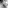
\includegraphics[width=0.1\textwidth]{figures/3.png} \\ \vspacemip
	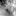
\includegraphics[width=0.2\textwidth]{figures/4.png} \\ \vspacemip
	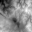
\includegraphics[width=0.4\textwidth]{figures/5.png} \\ \vspacemip
	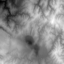
\includegraphics[width=0.8\textwidth]{figures/6.png}
	\caption{An example of the~averaging used to produce mip-maps; each mip-map is produced from the~previous larger one by averaging of each four neighboring pixels. The~brighter a~pixel, the~higher point it represents.}
	\label{fig:averaging}
\end{figure}

\section{Top-down pass}\label{sec:top-down}
This pass is performed in the~offline compression after the~first bottom-up pass, in which case it computes the~residuals $\objdot{E}{0..n}$ needed to completely progressively reconstruct the~compressed multiresolution representation of the~input $\lnorm{n}$. During the~following real-time decompression, this is the~only pass which is performed, with the~only difference that it no longer computes the~residuals, but it just reads them and uses them to reconstruct the~data. Let us describe it in detail, so that it becomes clear how this pass is implemented.

In the~previous chapter describing the~outline of the~method, we claimed that we construct a~larger decompressed mip-map $\ldot{i+1}$ from the~smaller $\ldot{i}$ in just one step (eq.~\ref{eq:nextLevel}). This is not exacly true, it is a~simplification which we made for several reasons: to give the~reader a~simple high-level idea of the~method, to make the~fact that $maxdev(\ldot{i+1}, \lnorm{i+1}) < \objnorm{D}{}$ easier to see and to make it clear that the~way the~target mip-maps $\lnorm{n-1..0}$ look has no effect on this constraint. However, the~truth is that to get $\ldot{i+1}$ from $\ldot{i}$, the~prediction operator $\opnorm{P}{}$ is applied consecutively three times. Its form is different at each of these applications which reflects the~fact that before each application, different height values are known - the~later the~application, the~more values are known. After each of these applications, the~residuals are computed during the~compression and added to~the already computed values during both the~compression and decompression. Nevertheless, the~two main principles which ensure that the~maximum error bound between $\lnorm{i+1}$ and $\ldot{i+1}$ is kept remain unchanged - during the~compression, the~residuals are still computed against the~target mip-map $\lnorm{i+1}$ after each application of $\opnorm{P}{}$ and all predictions are made from the~reconstructed values which ensures that both the~compression and the~decompression add the~residuals to the~same values. Hence, let us explain how these three steps are performed.

 When constructing the~larger compressed mip-map $\ldot{i+1}$ from $\ldot{i}$, we can imagine it as every pixel $p$ from $\ldot{i}$ being substituted by four pixels $a, b, c, d$ in $\ldot{i+1}$ as depicted in Fig.~\ref{fig:subst}. This substitution is the~exact inverse of the~one performed in the~first bottom-up pass described in the~previous section ???. We will apply the~prediction operator and subsequent residuals computation and addition three times in order to compute the~values of the~four pixels and the~residuals needed to reconstruct them from $p$ during the~decompression.

\begin{figure}
	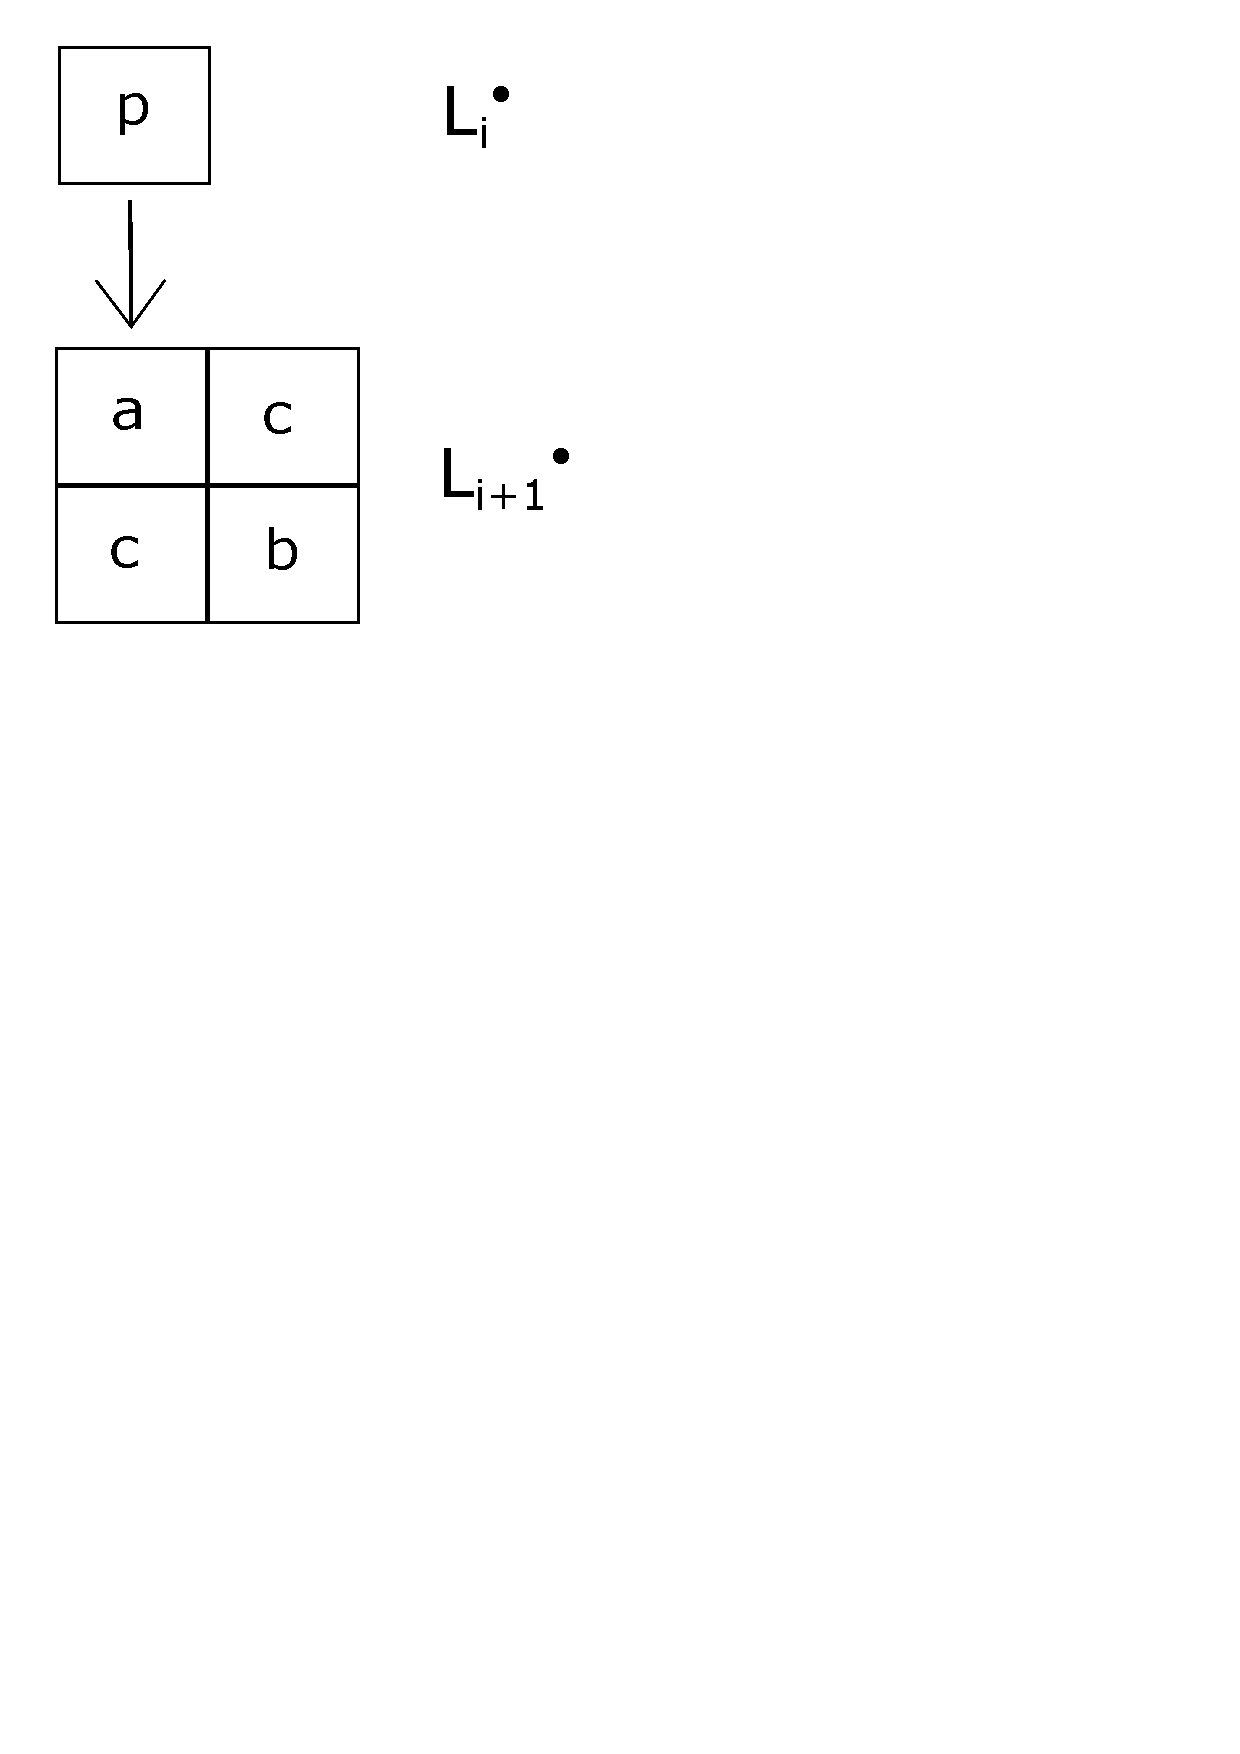
\includegraphics[trim={0 19cm 11cm 0}, clip, width=0.28\textwidth]{figures/subst.pdf}\centering
	\caption{Substituting the~pixel p in $\ldot{i}$ with four pixels in $\ldot{i+1}$}
	\label{fig:subst}
\end{figure}
In the~first of the~three steps, we compute the~pixels labeled $a$. To predict them from their corresponding $p$ pixels inside $\ldot{i}$, we use a~simple prediction operator $\opnorm{P}{a}(\ldot{i}) = p$. We compute the~residuals $\objnorm{E}{a}$ and $\objdot{E}{a}$ with respect to the~target value $a_t$ in $\lnorm{i+1}$ and then assign $a$ the~final value $a\bullet$ (eq. \ref{eq:a}, recall that $\opnorm{Q}{D}$ is a~uniform quantizer respecting the~maximum deviation $D$: $maxdev(v, \opnorm{Q}{D}(v)) < D$. It is clear that  $maxdev(a\bullet, a_{t}) \leq \objnorm{D}{}$. The~explanation would be the~same as in Chapter~\ref{chap:outline}.

$$\objnorm{E}{a} = a_t - p$$
$$\objdot{E}{a} = \opnorm{Q}{D}(\objnorm{E}{a})$$
\begin{equation}
\label{eq:a}
a\bullet = p + \objdot{E}{a}
\end{equation}

In the~second of the~three steps, we compute the~pixels labeled $b$. We do not predict them from $\ldot{i}$ anymore, but from the~already available pixels $a\bullet$ inside $\ldot{i+1}$. The~prediction operator $\opnorm{P}{b}$ used for this has now the~form of a~straight-oriented Neville interpolating filter of order 2. All it does is that when it is requested to predict the~height at some pixel, it just averages the~heights of its certain four neighboring pixels as depicted in Fig.~\ref{fig:bcomp}. It is easy to see that as long as it is requested to predict the~height at pixels $b$, it always averages only the~already known $a\bullet$ pixels. This is the~same prediction operator as the~one used in C-BDAM to predict the~heights of the~samples located at the~border of a~LOD hierarchy node. Once the~predictions of $b$ pixels are known, we perform an~analogic computation of residuals $\objnorm{E}{b}$ and their quantizations $\objdot{E}{b}$, again with respect to the~corresponding target values $b_t$ in $\lnorm{i+1}$. Finally, we assign $b$ its final value $b\bullet$ (eq.~\ref{eq:b}).

\begin{figure}
	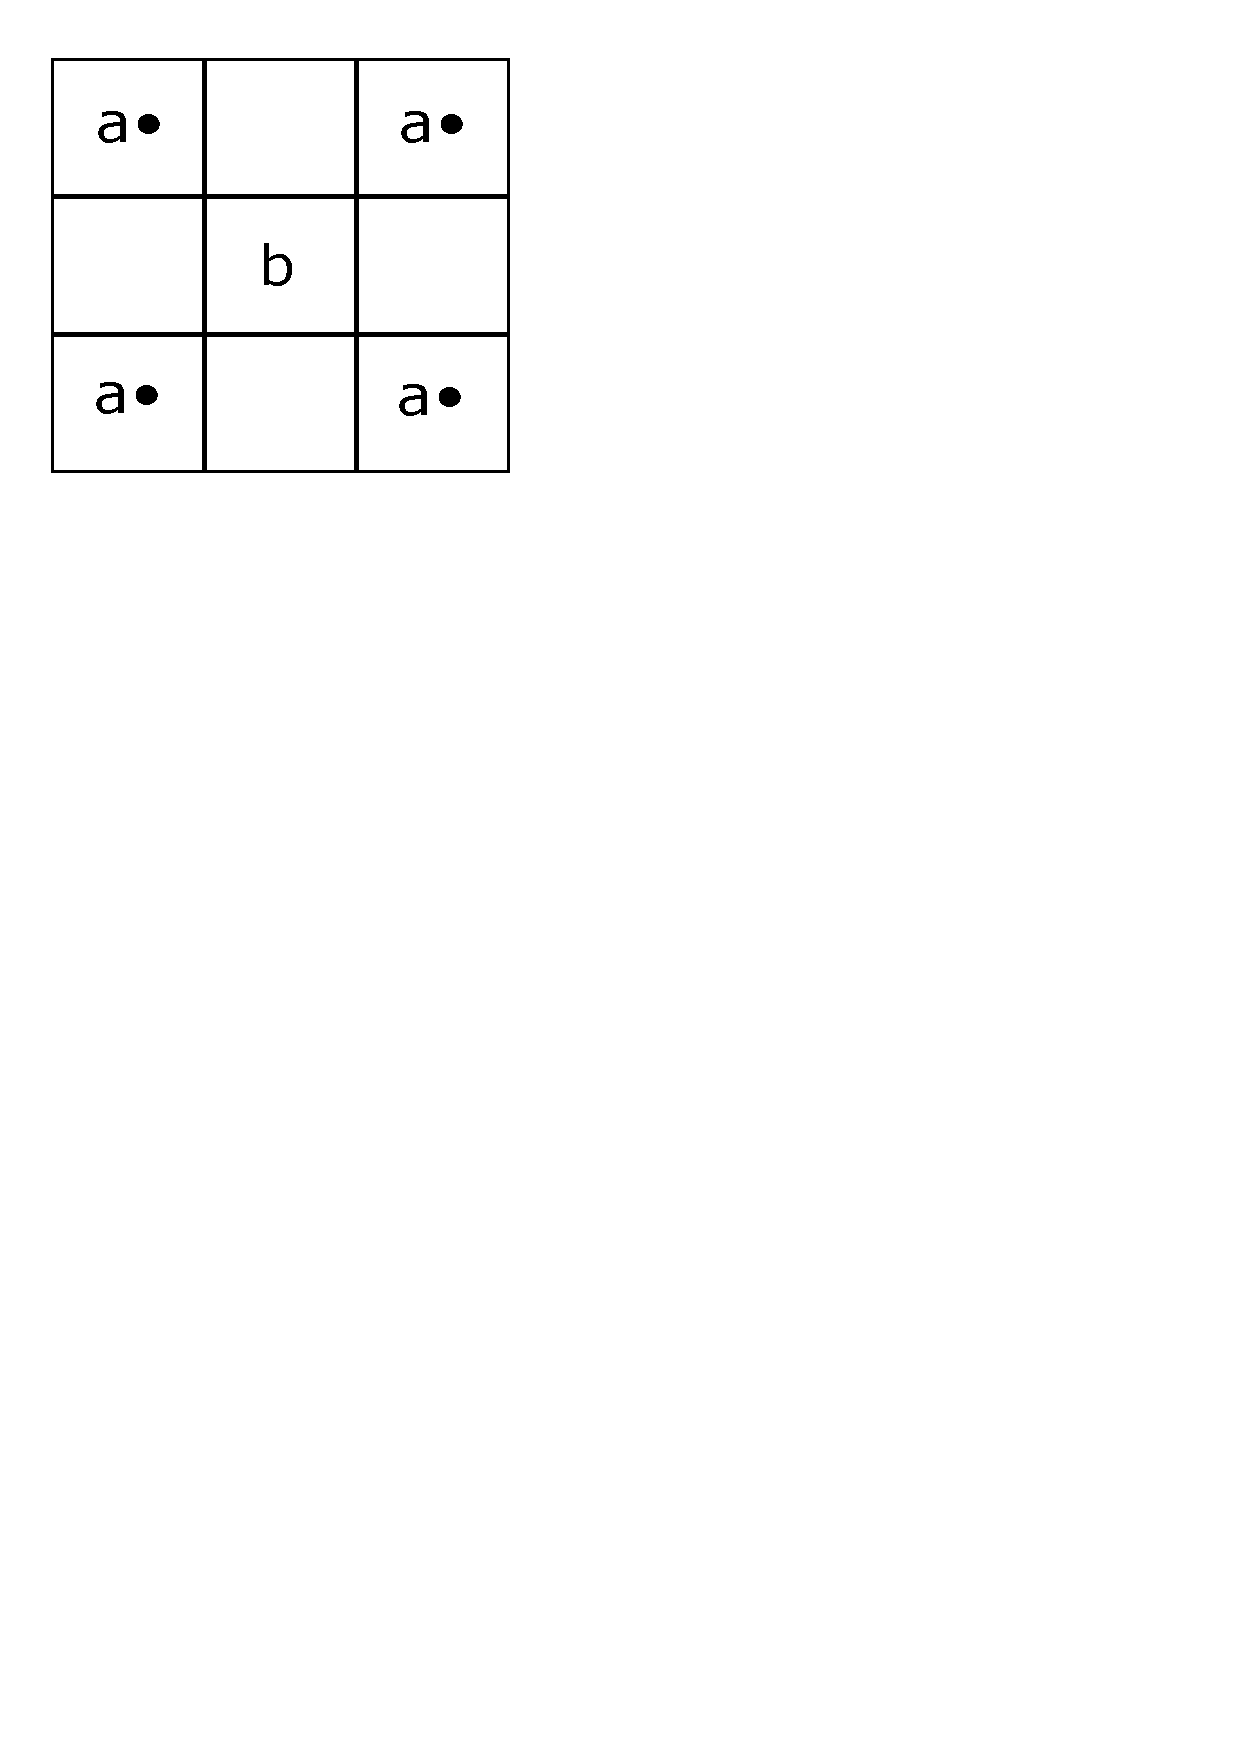
\includegraphics[trim={0 21cm 10cm 0}, clip, width=0.3\textwidth]{figures/bcomp.pdf}\centering
	\caption{The~prediction operator of $b$ - $\opnorm{P}{b}(\ldot{i+1})$ - averages the~compressed heights at all the~displayed $a\bullet$.}
	\label{fig:bcomp}
\end{figure}

$$\objnorm{E}{b} = b_t - \opnorm{P}{b}(\ldot{i+1})$$
$$\objdot{E}{b} = \opnorm{Q}{D}(\objnorm{E}{b})$$
\begin{equation}
\label{eq:b}
b\bullet = \opnorm{P}{b}(\ldot{i+1}) + \objdot{E}{b}
\end{equation}

The~reason why C-BDAM uses the~order 2 Neville interpolating filter at the~borders is that thanks to the~way the~samples are organized inside a~node of its LOD hierarchy, the~filter does not pick the~samples behind the~node's border. We can view the~mip-map in our method as an analogy to the~node in C-BDAM. However, the~spatial organization of mip-map samples in our method differs from the~organization of samples inside a~LOD node in C-BDAM, so unlike in C-BDAM, in our method it might happen that this interpolating filter comes out of the~underlying mip-map. We handle this by only including the~valid interior values in the~resulting average and completely ignoring the~imaginary values behind the~mip-map borders. Thus, when computing a~certain prediction, we count how many times the~filter has hit the~interior of mip-map and divide the~sum of the~valid interior heights with this number of hits. Most of the~times, the~number of hits will be 4, but it will be 2 at the~borders and just 1 at the~corners. This way, it is always ensured that the~filter does not make any data up, unlike the~possible alternative of some mirror extension of data behind the~borders. ??? Comparison with mirror extension ???

C-BDAM uses the~larger order 4 Neville interpolating filter to predict the~heights at the~interior of a~node of its LOD hierarchy. This filter covers larger area - it samples twelve points instead of four. In addition, it does not compute the~average of these points, but their weighted sum. Just like in the~case of simple averaging, the~sum of the~weights is 1. The~difference is that the~four closest points have a~certain positive weight, whereas the~remaining eight further points have a~different negative weight, the~absolute value of which is lower than the~first weight (Fig.~???). The~property with the~lower absolute value indicates that the~points which are further affect the~result less. The~fact that their weights are negative basically means that the~valleys and hills are predicted better (Fig.~???). 

Unlike C-BDAM, this method uses the~smaller order 2 filter even for the~interior samples. Let us explain the~reasons why we decided to do so. The~first reason is the~increase of speed. The~order 2 filter only averages four values, whereas the~order 4 filter averages 12 values. Moreover, the~subsequent averaging performed by the~order 2 filter can easily be cached during the~horizontal traversal which is an~additional reduction of the~computation overhead (Fig.~???). We also tried using the~order 4 filter with various weights settings for the~interior values, too. This slightly increased the~compression ratio - probably because this~filter is better at predicting hills and walleys - but worsened the~quality of compression by producing more significant artifacts near smooth terrain's borders (Fig.~\ref{fig:artifs_border}) and sharp terrain transitions (Fig.~\ref{fig:artifs_sharp_change}). The~most probable cause of this is that the~predictions made by the~order 4 filter tend to differ from the~neighboring heights more. This emphasises the~artifacts.

\newcommand{\incimg}[3]{\includegraphics[width=#1px, height=#2px]{#3}}
\newcommand{\incartifborder}[1]{\incimg{95}{70}{#1}}

\begin{figure}
	Original \incartifborder{figures/artif_orig0.png}
	\incartifborder{figures/artif_orig1.png}\\
	Order 2~~\incartifborder{figures/artif_four0.png}
	\incartifborder{figures/artif_four1.png}\\
	Order 4~~\incartifborder{figures/artif_twelve0.png}
	\incartifborder{figures/artif_twelve1.png}\\
	\caption{Two examples of the~difference between artifacts caused by order 2 and order 4 filters near smooth terrain's border - in the~first row there are the~target heightmaps, in the~second, there are the~same heightmaps compressed using the~order 2 filter, in the~third row, the~heightmaps compressed with the~order 4 filter.}
	\label{fig:artifs_border}
\end{figure}

\newcommand{\incartifchange}[1]{\incimg{95}{95}{#1}}

\begin{figure}
	Original \incartifchange{figures/artif_change_orig0.png}
	\incartifchange{figures/artif_change_orig1.png}\\
	Order 2~~\incartifchange{figures/artif_change_four0.png}
	\incartifchange{figures/artif_change_four1.png}\\\
	Order 4~~\incartifchange{figures/artif_change_twelve0.png}
	\incartifchange{figures/artif_change_twelve1.png}\\
	\caption{Two examples of the~difference between artifacts caused by order 2 and order 4 filters near a~sharp terrain change - in the~first row there are the~target heightmaps, in the~second row, the~same heightmaps compressed using the~order 2 filter, in the~third row, the~heightmaps compressed with the~order 4 filter. The~span of the~values in the~original images is from 0 to 16 and the~maximum absolute deviation ($D$) of compression is set to 9.}
	\label{fig:artifs_sharp_change}
\end{figure}

Generally, the~reason why these artifacts occur is that as long as the~predictions are close enough to the~target mip-map and their quantized residuals are equal to zero, the~compressed values might remain above/under the~terrain for a~long time, but only until one prediction gets a~bit further from the~target terrain. As soon as it happens, its associated residual will be quantized to a~certain non-zero value which will result in the~reconstructed value being flipped to the~opposite side of the~real terrain which produces a~visual artifact. It is not a~coincidence that this often occurs near a~sharp change in the~terrain. The~predictions produced by the~averaging filter get a~bit different from the~adjacent ones near this change, because at these places, the~filter reaches out to the~area behind the~change (Fig.~\ref{fig:artifs_theory}). This difference might then cause the difference in residuals - the~quantized residuals further from this change might be all zeroes, whereas the~residual near this change not, causing a~spike to occur. This spike will then get propagated to the~following compressed mip-map levels. The~only thing that is guaranteed is that the~maximum error bound is still satisfied. ???(musim overit, clipping je nasadeny len v Bohemke, ale je to lepsi napad ako mirroring, tusim, ze to aj zlepsilo kompresny pomer, no nezistoval som pri nom, ake su artefakty)The~clipping performed by the~predicting filter near the~mip-map borders creates the~effect similar to a~sharp terrain change, too, in a~bit different way - by the~sole fact that the~terrain behind the~border no longer follows its trend up to the~border (rising, for example), but is practically mirrored behind the~border (following the~example, falling), because instead of reaching out to the~non-existing values out of the~mip-map, the~existing ones are used.???

\begin{figure}
	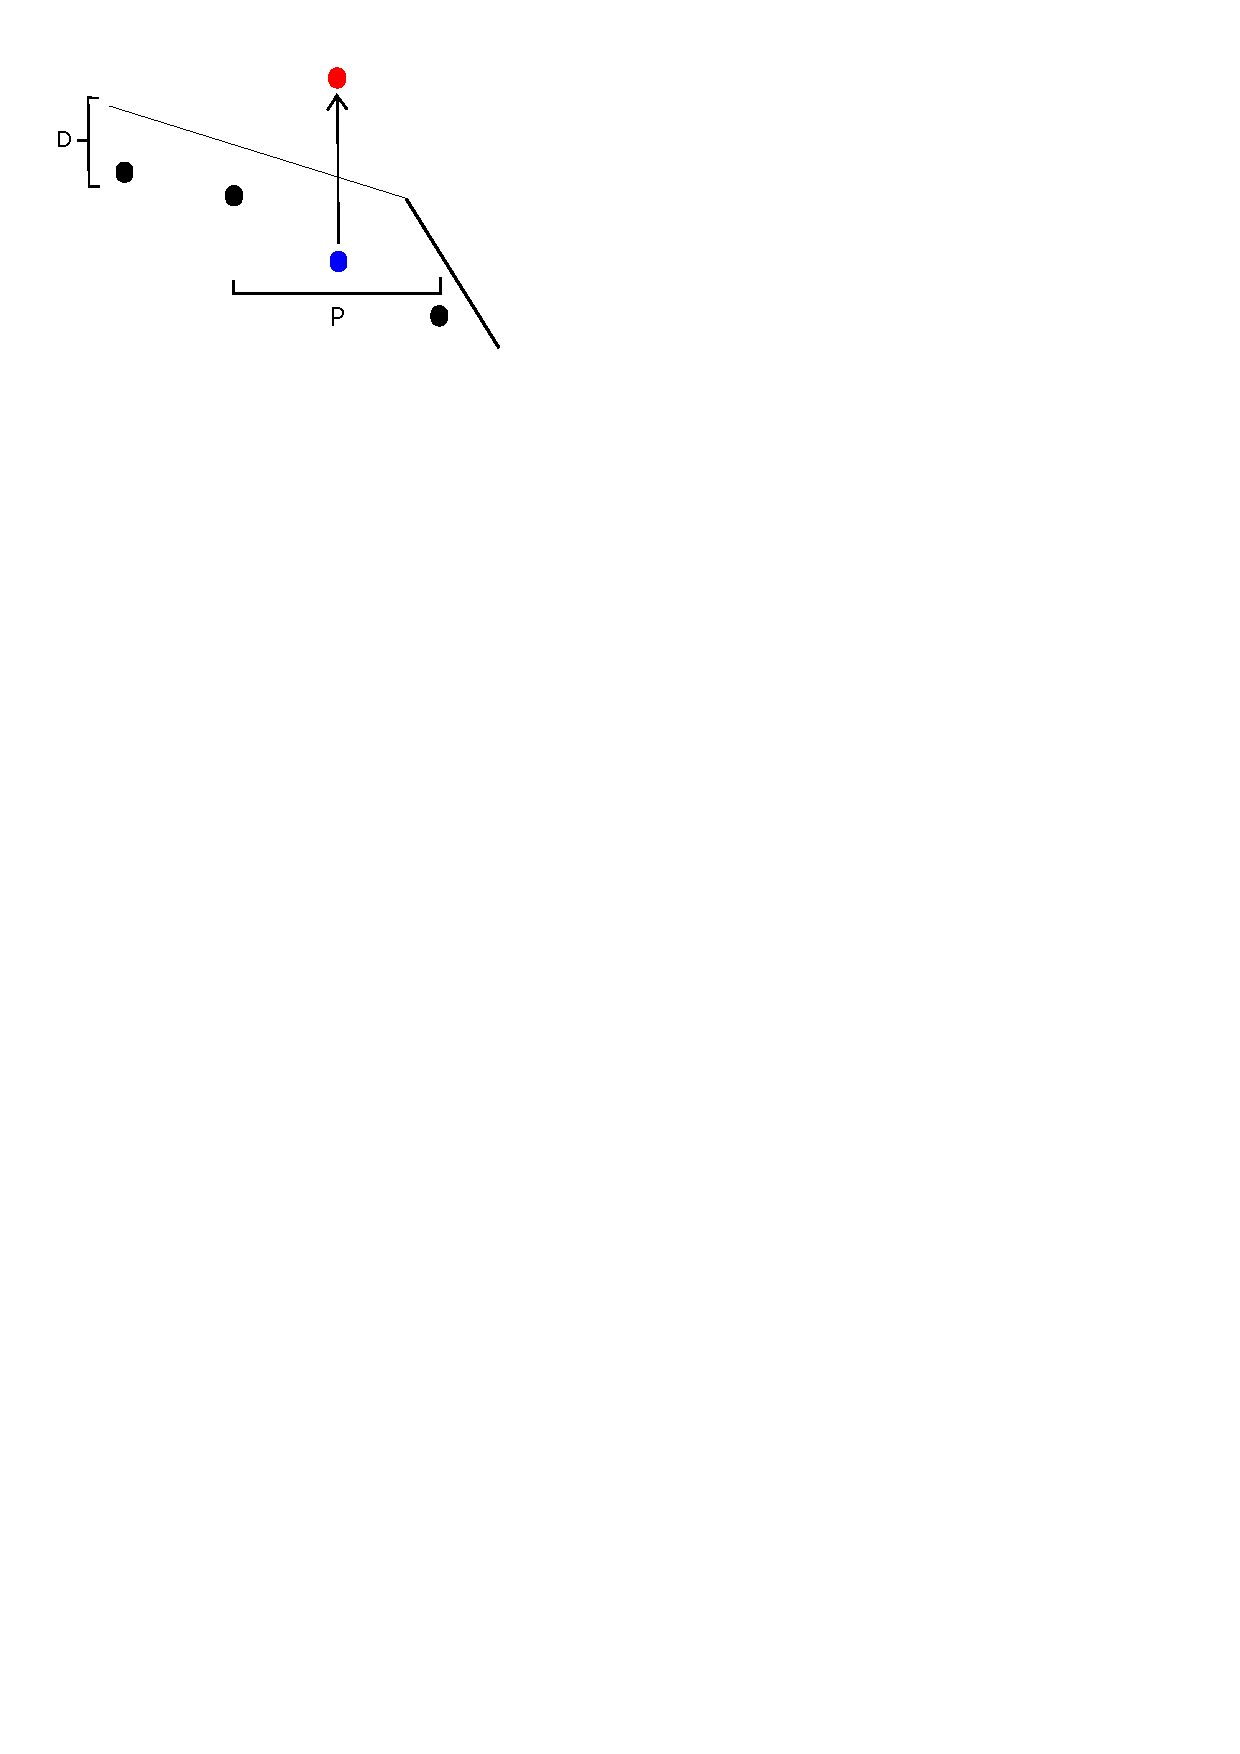
\includegraphics[trim={0 24cm 7cm 0}, clip, width=0.45\textwidth]{figures/artifs_theory.pdf}\centering
	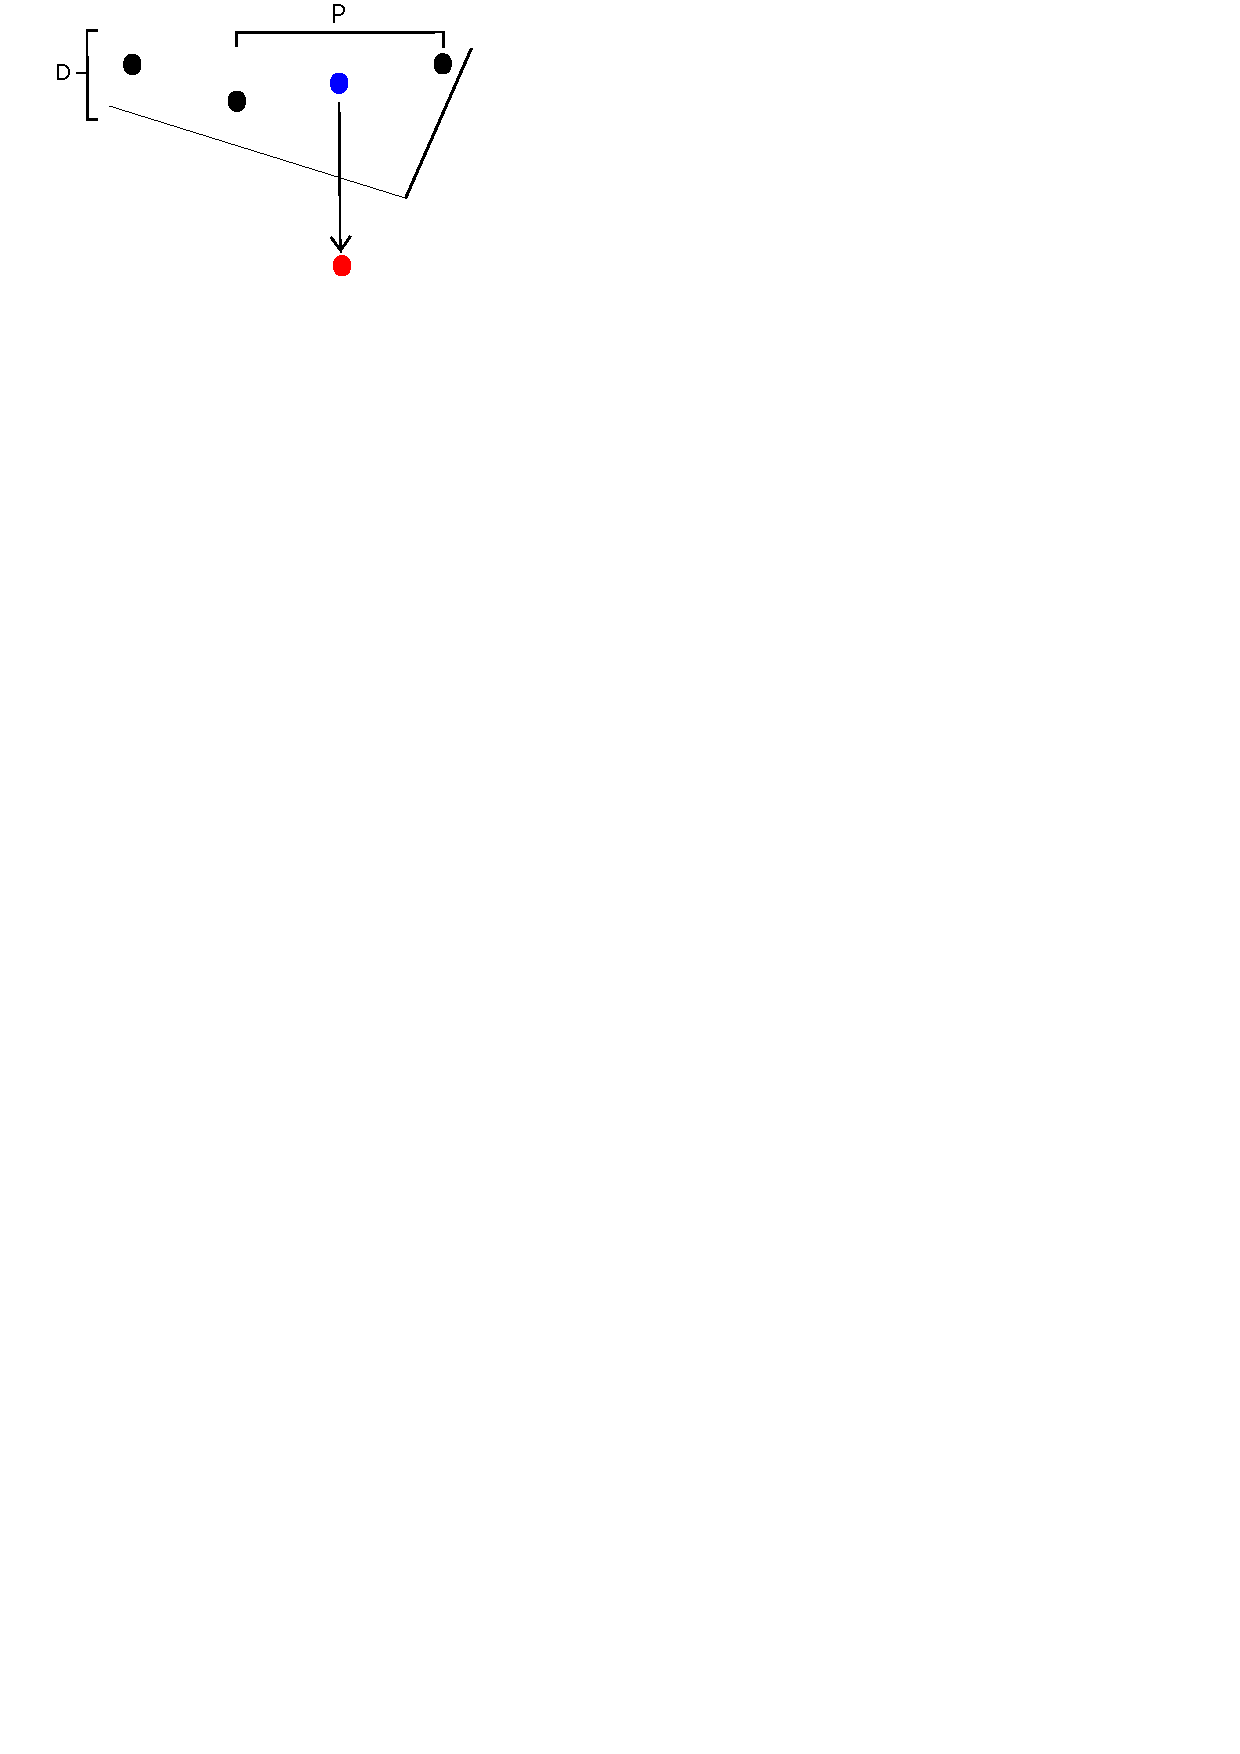
\includegraphics[trim={0 24cm 7cm 0}, clip, width=0.45\textwidth]{figures/artifs_theory2.pdf}\centering
	\caption{Two illustrations of how artifacts can occur near sharp terrain changes - the~black dots stand for the~predictions which are still within the~maximum-error bound $D$ from the~target terrain, the~blue dots represent the~predictions which are just slightly further from the~terrain, because their filters span to the~area behind the~change. Due to the~fact that a~uniform quantizer with the~step of $2D-1$ is applied to the~residuals, the~residuals added to the~blue predictions will cause them to be shifted by $2D - 1$ to the~top (the~image on the~left) or to the~bottom (the~image on the~right), creating sharp peaks in the~reconstructed values - the~artifacts.}
	\label{fig:artifs_theory}
\end{figure}

In the~last of the~three steps, we compute the~pixels labeled $c$. We predict them from the~already available compressed values of both $a\bullet$ and $b\bullet$ inside $\ldot{i+1}$. The~prediction operator $\opnorm{P}{c}$ used for it has now the~form of a~diagonally-oriented Neville interpolating filter of order 2. It is the~same as the~previously applied $\opnorm{P}{b}$, except for its different orientation - relatively to $\opnorm{P}{b}$, it is rotated by 45 degrees and averages the~4-connected neighbors of the~point of application (Fig.~\ref{fig:ccomp}). Once the~predictions of heights at $c$ pixels are known, we perform an~analogic computation of residuals $\objnorm{E}{c}$ and their quantizations $\objdot{E}{c}$, again with respect to the~corresponding target values $c_t$ inside $\lnorm{i+1}$. At last, we assign every pixel $c$ its final value $c\bullet$ (eq.~\ref{eq:c}).

\begin{figure}
	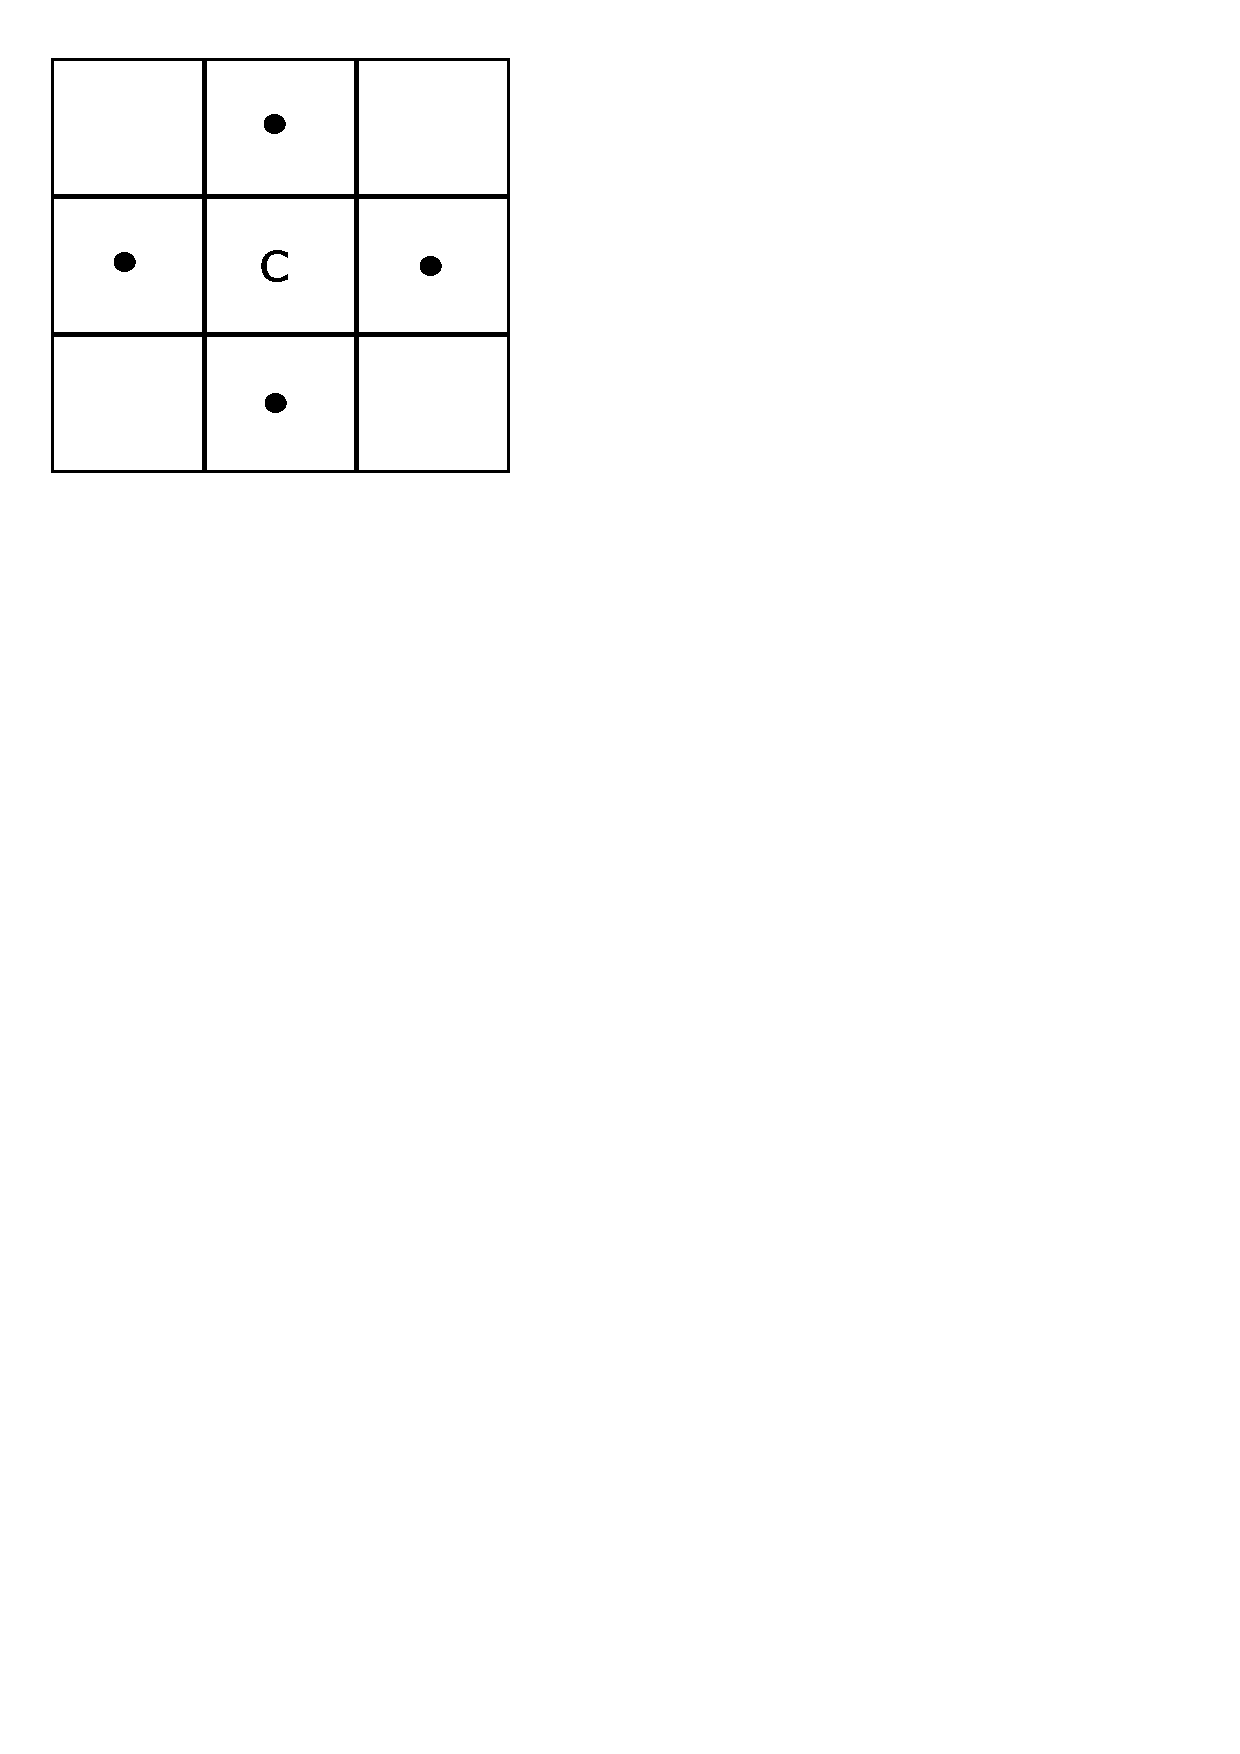
\includegraphics[trim={0 21cm 10cm 0}, clip, width=0.3\textwidth]{figures/ccomp.pdf}\centering
	\caption{The~prediction operator of $c$ - $\opnorm{P}{c}(\ldot{i+1})$ - averages the~compressed heights at all the~pixels marked with a~dot - $\bullet$. Both $a\bullet$ and $b\bullet$ are among these pixels.}
	\label{fig:ccomp}
\end{figure}

$$\objnorm{E}{c} = c_t - \opnorm{P}{c}(\ldot{i+1})$$
$$\objdot{E}{c} = \opnorm{Q}{D}(\objnorm{E}{c})$$
\begin{equation}
\label{eq:c}
c\bullet = \opnorm{P}{c}(\ldot{i+1}) + \objdot{E}{c}
\end{equation}

Just like in the~case of $\opnorm{P}{b}$, $\opnorm{P}{c}$ can reach out behind the~mip-map borders, too. We handled these situations exacly the~same way - we only average the~heights which are inside the~mip-map (Fig.~\ref{fig:cborders}). Similarly to the~predictions of $b$ pixels, we use the~order 2 filter to predict the~heights at all $c$ pixels - even the~interior ones. The~subsequent predictions of neighboring $c$ pixels can again be cached to spare some computations. However, the~traversal with $\opnorm{P}{c}$ must now be diagonal in order to make such caching possible (Fig.~???).

\begin{figure}
	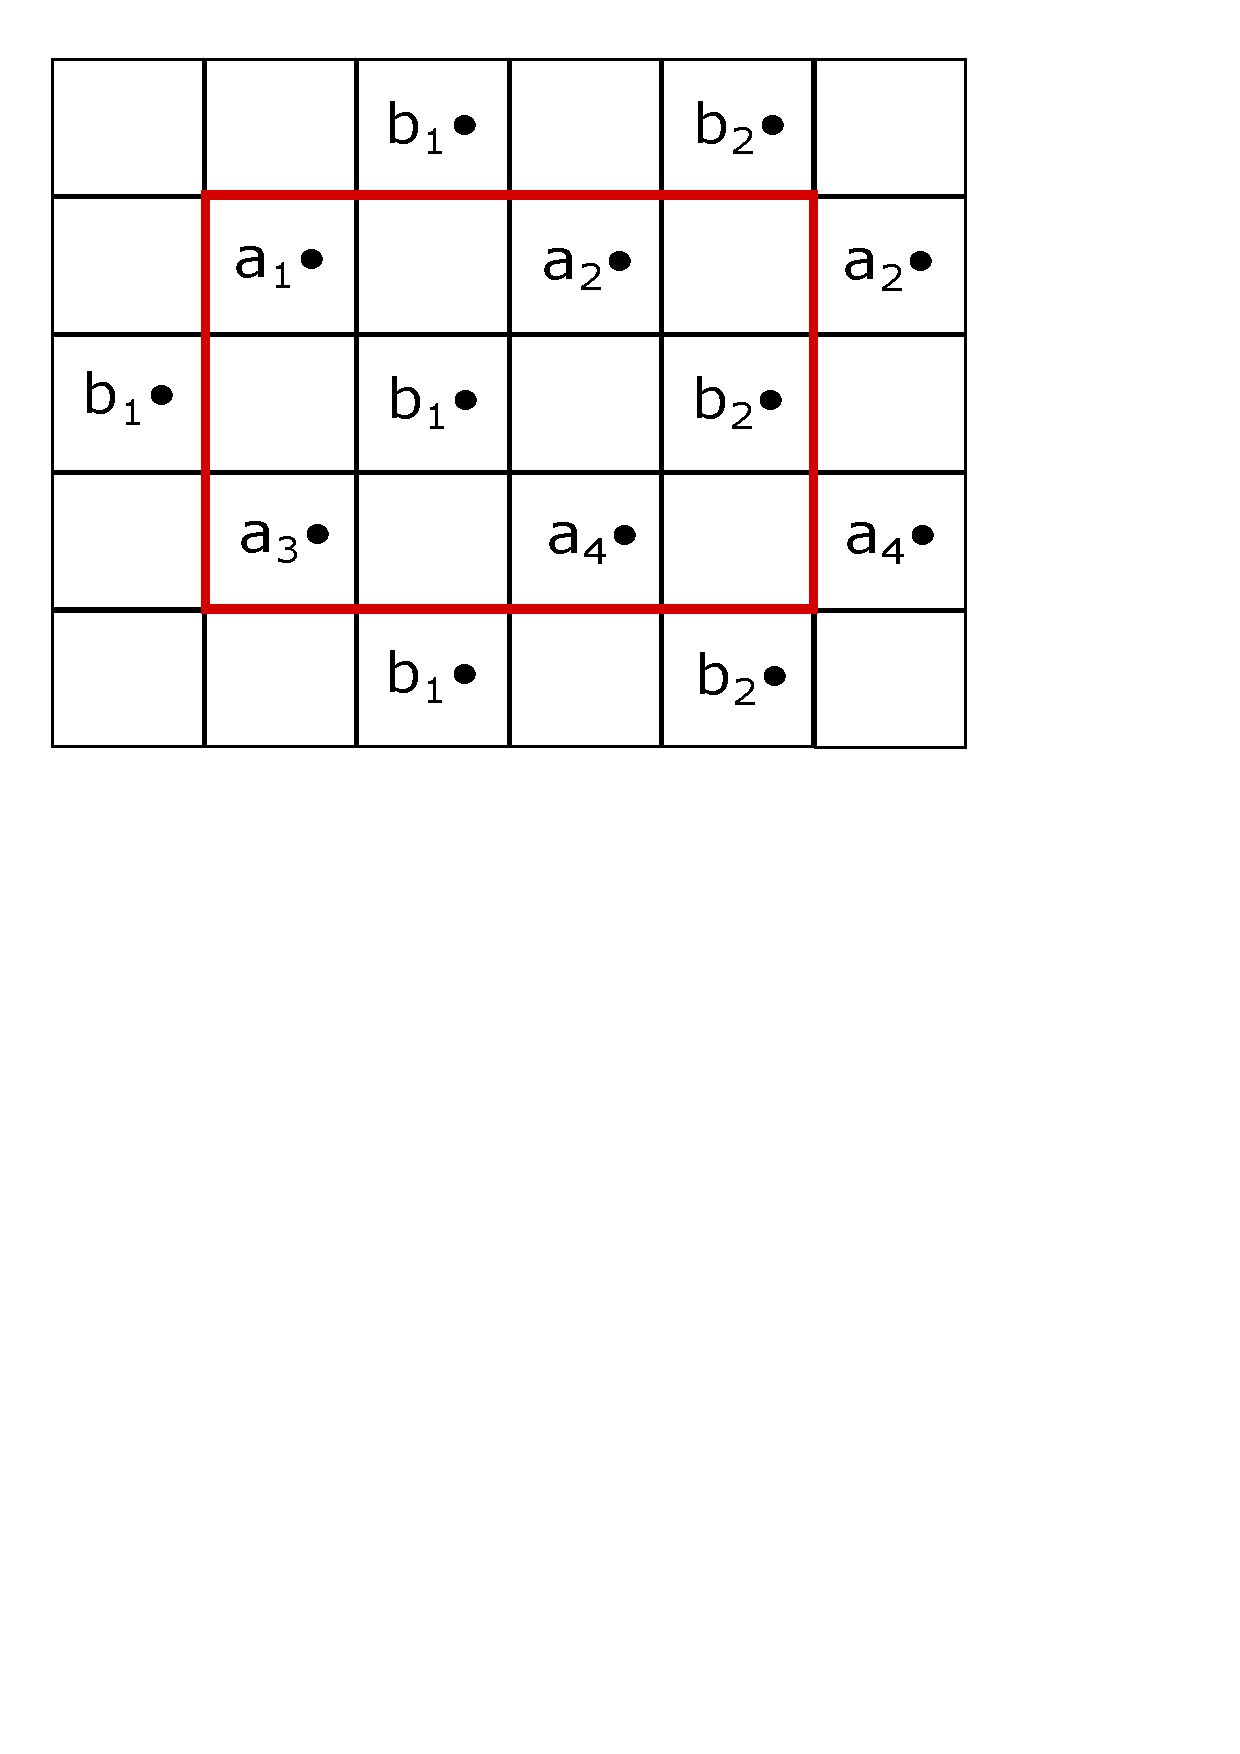
\includegraphics[trim={0 17cm 3cm 0}, clip, width=0.45\textwidth]{figures/extc.pdf}\centering
	\caption{(!!!aktualizuj)Handling of border cases in the~computation of $\opnorm{P}{c}(\ldot{i+1})$ - the~red line represents the~border.}
	\label{fig:cborders}
\end{figure}

Now, let us sum up what we have already done in a~few sentences. We have performed all the~three subsequent applications of the~prediction operator in different forms - $\opnorm{P}{a}$, $\opnorm{P}{b}$ and $\opnorm{P}{c}$ on the~already computed compressed heights in order to obtain the~predictions of the~yet unknown heights. After each of these applications, we calculated the~differences between the~predictions and the~target values located at the~target mip-map at the~same places, obtaining the~raw residuals $\objnorm{E}{a}$, $\objnorm{E}{b}$ and $\objnorm{E}{c}$. Then we quantized these residuals with $\opnorm{Q}{D}$ - the~uniform quantizer respecting the~maximum deviation $D$ which ensures that when the~quantized residuals are added back to the~predictions, all these~summations will be within the~deviation $D$ from the~corresponding target heights. We called the~quantized residuals $\objdot{E}{a}$, $\objdot{E}{b}$ and $\objdot{E}{c}$. Together, they form $\objdot{E}{i+1}$ - all the~residuals required to reconstruct the~larger compressed mip-map $\ldot{i+1}$ from the~previous compressed $\ldot{i}$.

 Finally, with all the~quantized residuals computed, we losslessly compress them and store them. We firstly compress and store $\objdot{E}{0} = \opnorm{Q}{D}(\lnorm{0})$, then $\objdot{E}{1}$, up to $\objdot{E}{n}$. Thanks to this organization, when we want to run-time decompress any $\ldot{i}$, we will be required to read just the~starting continuous block of the~compressed data $\objdot{E}{0..i}$. This is called the~progressive decompression. The~decompression itself is performed in a~similar way. The~only difference is that the~quantized residuals are no longer calculated, but just read and decompress. Thus, with $\ldot{i}$ available, we obtain $\ldot{i+1}$ by substituting every pixel labeled $p$ inside $\ldot{i}$ by four neighboring pixels labeled $a$, $b$, $c$ in $\ldot{i+1}$ (Fig.~\ref{fig:subst}), the~heights of which will then be computed in three steps. At each of these steps, we will just predict the~heights of the~pixels with the~relevant prediction operator. This will be followed only by adding the~read and decompressed residuals  to the~predictions (the~last lines of eq.~\ref{eq:a}, \ref{eq:b}, \ref{eq:c}).
 
  The~lossless compression of residuals is performed in two steps - packing followed by lossless compression by Zlib. During packing, we divide all the~residuals with their quantization interval. Then, we shift them, so that all the~values are non-negative. Then, we crop the~number of bits of each residual to the~number of bits of the~largest value. Obviously, we also store the~information needed to perform the~inverse of packing in the~reconstruction - the~quantization interval and the~upper-shift amount. Only after this packing are the~residuals losslessly encoded by Zlib. The~packing proved to be useful, as it additionally increased the~compression ratio. The~decompression is just the~inverse - lossless decompression by Zlib followed by the~unpacking - expanding the~residuals back into floats, shifting them down by the~shifting amount and multiplying them with the~quantization interval.
